%% bare_adv.tex
%% V1.4b
%% 2015/08/26
%% by Michael Shell
%% See:
%% http://www.michaelshell.org/
%% for current contact information.
%%
%% This is a skeleton file demonstrating the advanced use of IEEEtran.cls
%% (requires IEEEtran.cls version 1.8b or later) with an IEEE Computer
%% Society journal paper.
%%
%% Support sites:
%% http://www.michaelshell.org/tex/ieeetran/
%% http://www.ctan.org/pkg/ieeetran
%% and
%% http://www.ieee.org/

%%*************************************************************************
%% Legal Notice:
%% This code is offered as-is without any warranty either expressed or
%% implied; without even the implied warranty of MERCHANTABILITY or
%% FITNESS FOR A PARTICULAR PURPOSE!
%% User assumes all risk.
%% In no event shall the IEEE or any contributor to this code be liable for
%% any damages or losses, including, but not limited to, incidental,
%% consequential, or any other damages, resulting from the use or misuse
%% of any information contained here.
%%
%% All comments are the opinions of their respective authors and are not
%% necessarily endorsed by the IEEE.
%%
%% This work is distributed under the LaTeX Project Public License (LPPL)
%% ( http://www.latex-project.org/ ) version 1.3, and may be freely used,
%% distributed and modified. A copy of the LPPL, version 1.3, is included
%% in the base LaTeX documentation of all distributions of LaTeX released
%% 2003/12/01 or later.
%% Retain all contribution notices and credits.
%% ** Modified files should be clearly indicated as such, including  **
%% ** renaming them and changing author support contact information. **
%%*************************************************************************


% *** Authors should verify (and, if needed, correct) their LaTeX system  ***
% *** with the testflow diagnostic prior to trusting their LaTeX platform ***
% *** with production work. The IEEE's font choices and paper sizes can   ***
% *** trigger bugs that do not appear when using other class files.       ***                          ***
% The testflow support page is at:
% http://www.michaelshell.org/tex/testflow/


% IEEEtran V1.7 and later provides for these CLASSINPUT macros to allow the
% user to reprogram some IEEEtran.cls defaults if needed. These settings
% override the internal defaults of IEEEtran.cls regardless of which class
% options are used. Do not use these unless you have good reason to do so as
% they can result in nonIEEE compliant documents. User beware. ;)
%
%\newcommand{\CLASSINPUTbaselinestretch}{1.0} % baselinestretch
%\newcommand{\CLASSINPUTinnersidemargin}{1in} % inner side margin
%\newcommand{\CLASSINPUToutersidemargin}{1in} % outer side margin
%\newcommand{\CLASSINPUTtoptextmargin}{1in}   % top text margin
%\newcommand{\CLASSINPUTbottomtextmargin}{1in}% bottom text margin




%
\documentclass[10pt,journal,compsoc]{IEEEtran}
% If IEEEtran.cls has not been installed into the LaTeX system files,
% manually specify the path to it like:
% \documentclass[10pt,journal,compsoc]{../sty/IEEEtran}


% For Computer Society journals, IEEEtran defaults to the use of
% Palatino/Palladio as is done in IEEE Computer Society journals.
% To go back to Times Roman, you can use this code:
%\renewcommand{\rmdefault}{ptm}\selectfont





% Some very useful LaTeX packages include:
% (uncomment the ones you want to load)



% *** MISC UTILITY PACKAGES ***
%
%\usepackage{ifpdf}
% Heiko Oberdiek's ifpdf.sty is very useful if you need conditional
% compilation based on whether the output is pdf or dvi.
% usage:
% \ifpdf
%   % pdf code
% \else
%   % dvi code
% \fi
% The latest version of ifpdf.sty can be obtained from:
% http://www.ctan.org/pkg/ifpdf
% Also, note that IEEEtran.cls V1.7 and later provides a builtin
% \ifCLASSINFOpdf conditional that works the same way.
% When switching from latex to pdflatex and vice-versa, the compiler may
% have to be run twice to clear warning/error messages.






% *** CITATION PACKAGES ***
%
\ifCLASSOPTIONcompsoc
  % The IEEE Computer Society needs nocompress option
  % requires cite.sty v4.0 or later (November 2003)
  \usepackage[nocompress]{cite}
\else
  % normal IEEE
  \usepackage{cite}
\fi
% cite.sty was written by Donald Arseneau
% V1.6 and later of IEEEtran pre-defines the format of the cite.sty package
% \cite{} output to follow that of the IEEE. Loading the cite package will
% result in citation numbers being automatically sorted and properly
% "compressed/ranged". e.g., [1], [9], [2], [7], [5], [6] without using
% cite.sty will become [1], [2], [5]--[7], [9] using cite.sty. cite.sty's
% \cite will automatically add leading space, if needed. Use cite.sty's
% noadjust option (cite.sty V3.8 and later) if you want to turn this off
% such as if a citation ever needs to be enclosed in parenthesis.
% cite.sty is already installed on most LaTeX systems. Be sure and use
% version 5.0 (2009-03-20) and later if using hyperref.sty.
% The latest version can be obtained at:
% http://www.ctan.org/pkg/cite
% The documentation is contained in the cite.sty file itself.
%
% Note that some packages require special options to format as the Computer
% Society requires. In particular, Computer Society  papers do not use
% compressed citation ranges as is done in typical IEEE papers
% (e.g., [1]-[4]). Instead, they list every citation separately in order
% (e.g., [1], [2], [3], [4]). To get the latter we need to load the cite
% package with the nocompress option which is supported by cite.sty v4.0
% and later.





% *** GRAPHICS RELATED PACKAGES ***
%
\ifCLASSINFOpdf
\usepackage[pdftex]{graphicx}
  % declare the path(s) where your graphic files are
   \graphicspath{{../pdf/}{../jpeg/}}
  % and their extensions so you won't have to specify these with
  % every instance of \includegraphics
   \DeclareGraphicsExtensions{.pdf,.jpeg,.png}
\else
  % or other class option (dvipsone, dvipdf, if not using dvips). graphicx
  % will default to the driver specified in the system graphics.cfg if no
  % driver is specified.
   \usepackage[dvips]{graphicx}
  % declare the path(s) where your graphic files are
   \graphicspath{{../eps/}}
  % and their extensions so you won't have to specify these with
  % every instance of \includegraphics
   \DeclareGraphicsExtensions{.eps}
\fi
% graphicx was written by David Carlisle and Sebastian Rahtz. It is
% required if you want graphics, photos, etc. graphicx.sty is already
% installed on most LaTeX systems. The latest version and documentation
% can be obtained at:
% http://www.ctan.org/pkg/graphicx
% Another good source of documentation is "Using Imported Graphics in
% LaTeX2e" by Keith Reckdahl which can be found at:
% http://www.ctan.org/pkg/epslatex
%
% latex, and pdflatex in dvi mode, support graphics in encapsulated
% postscript (.eps) format. pdflatex in pdf mode supports graphics
% in .pdf, .jpeg, .png and .mps (metapost) formats. Users should ensure
% that all non-photo figures use a vector format (.eps, .pdf, .mps) and
% not a bitmapped formats (.jpeg, .png). The IEEE frowns on bitmapped formats
% which can result in "jaggedy"/blurry rendering of lines and letters as
% well as large increases in file sizes.
%
% You can find documentation about the pdfTeX application at:
% http://www.tug.org/applications/pdftex





% *** MATH PACKAGES ***
%
%\usepackage{amsmath}
% A popular package from the American Mathematical Society that provides
% many useful and powerful commands for dealing with mathematics.
%
% Note that the amsmath package sets \interdisplaylinepenalty to 10000
% thus preventing page breaks from occurring within multiline equations. Use:
%\interdisplaylinepenalty=2500
% after loading amsmath to restore such page breaks as IEEEtran.cls normally
% does. amsmath.sty is already installed on most LaTeX systems. The latest
% version and documentation can be obtained at:
% http://www.ctan.org/pkg/amsmath





% *** SPECIALIZED LIST PACKAGES ***
%\usepackage{acronym}
% acronym.sty was written by Tobias Oetiker. This package provides tools for
% managing documents with large numbers of acronyms. (You don't *have* to
% use this package - unless you have a lot of acronyms, you may feel that
% such package management of them is bit of an overkill.)
% Do note that the acronym environment (which lists acronyms) will have a
% problem when used under IEEEtran.cls because acronym.sty relies on the
% description list environment - which IEEEtran.cls has customized for
% producing IEEE style lists. A workaround is to declared the longest
% label width via the IEEEtran.cls \IEEEiedlistdecl global control:
%
% \renewcommand{\IEEEiedlistdecl}{\IEEEsetlabelwidth{SONET}}
% \begin{acronym}
%
% \end{acronym}
% \renewcommand{\IEEEiedlistdecl}{\relax}% remember to reset \IEEEiedlistdecl
%
% instead of using the acronym environment's optional argument.
% The latest version and documentation can be obtained at:
% http://www.ctan.org/pkg/acronym


%\usepackage{algorithmic}
% algorithmic.sty was written by Peter Williams and Rogerio Brito.
% This package provides an algorithmic environment fo describing algorithms.
% You can use the algorithmic environment in-text or within a figure
% environment to provide for a floating algorithm. Do NOT use the algorithm
% floating environment provided by algorithm.sty (by the same authors) or
% algorithm2e.sty (by Christophe Fiorio) as the IEEE does not use dedicated
% algorithm float types and packages that provide these will not provide
% correct IEEE style captions. The latest version and documentation of
% algorithmic.sty can be obtained at:
% http://www.ctan.org/pkg/algorithms
% Also of interest may be the (relatively newer and more customizable)
% algorithmicx.sty package by Szasz Janos:
% http://www.ctan.org/pkg/algorithmicx




% *** ALIGNMENT PACKAGES ***
%
%\usepackage{array}
% Frank Mittelbach's and David Carlisle's array.sty patches and improves
% the standard LaTeX2e array and tabular environments to provide better
% appearance and additional user controls. As the default LaTeX2e table
% generation code is lacking to the point of almost being broken with
% respect to the quality of the end results, all users are strongly
% advised to use an enhanced (at the very least that provided by array.sty)
% set of table tools. array.sty is already installed on most systems. The
% latest version and documentation can be obtained at:
% http://www.ctan.org/pkg/array


%\usepackage{mdwmath}
%\usepackage{mdwtab}
% Also highly recommended is Mark Wooding's extremely powerful MDW tools,
% especially mdwmath.sty and mdwtab.sty which are used to format equations
% and tables, respectively. The MDWtools set is already installed on most
% LaTeX systems. The lastest version and documentation is available at:
% http://www.ctan.org/pkg/mdwtools


% IEEEtran contains the IEEEeqnarray family of commands that can be used to
% generate multiline equations as well as matrices, tables, etc., of high
% quality.


%\usepackage{eqparbox}
% Also of notable interest is Scott Pakin's eqparbox package for creating
% (automatically sized) equal width boxes - aka "natural width parboxes".
% Available at:
% http://www.ctan.org/pkg/eqparbox




% *** SUBFIGURE PACKAGES ***
%\ifCLASSOPTIONcompsoc
%  \usepackage[caption=false,font=footnotesize,labelfont=sf,textfont=sf]{subfig}
%\else
%  \usepackage[caption=false,font=footnotesize]{subfig}
%\fi
% subfig.sty, written by Steven Douglas Cochran, is the modern replacement
% for subfigure.sty, the latter of which is no longer maintained and is
% incompatible with some LaTeX packages including fixltx2e. However,
% subfig.sty requires and automatically loads Axel Sommerfeldt's caption.sty
% which will override IEEEtran.cls' handling of captions and this will result
% in non-IEEE style figure/table captions. To prevent this problem, be sure
% and invoke subfig.sty's "caption=false" package option (available since
% subfig.sty version 1.3, 2005/06/28) as this is will preserve IEEEtran.cls
% handling of captions.
% Note that the Computer Society format requires a sans serif font rather
% than the serif font used in traditional IEEE formatting and thus the need
% to invoke different subfig.sty package options depending on whether
% compsoc mode has been enabled.
%
% The latest version and documentation of subfig.sty can be obtained at:
% http://www.ctan.org/pkg/subfig




% *** FLOAT PACKAGES ***
%
%\usepackage{fixltx2e}
% fixltx2e, the successor to the earlier fix2col.sty, was written by
% Frank Mittelbach and David Carlisle. This package corrects a few problems
% in the LaTeX2e kernel, the most notable of which is that in current
% LaTeX2e releases, the ordering of single and double column floats is not
% guaranteed to be preserved. Thus, an unpatched LaTeX2e can allow a
% single column figure to be placed prior to an earlier double column
% figure.
% Be aware that LaTeX2e kernels dated 2015 and later have fixltx2e.sty's
% corrections already built into the system in which case a warning will
% be issued if an attempt is made to load fixltx2e.sty as it is no longer
% needed.
% The latest version and documentation can be found at:
% http://www.ctan.org/pkg/fixltx2e


%\usepackage{stfloats}
% stfloats.sty was written by Sigitas Tolusis. This package gives LaTeX2e
% the ability to do double column floats at the bottom of the page as well
% as the top. (e.g., "\begin{figure*}[!b]" is not normally possible in
% LaTeX2e). It also provides a command:
%\fnbelowfloat
% to enable the placement of footnotes below bottom floats (the standard
% LaTeX2e kernel puts them above bottom floats). This is an invasive package
% which rewrites many portions of the LaTeX2e float routines. It may not work
% with other packages that modify the LaTeX2e float routines. The latest
% version and documentation can be obtained at:
% http://www.ctan.org/pkg/stfloats
% Do not use the stfloats baselinefloat ability as the IEEE does not allow
% \baselineskip to stretch. Authors submitting work to the IEEE should note
% that the IEEE rarely uses double column equations and that authors should try
% to avoid such use. Do not be tempted to use the cuted.sty or midfloat.sty
% packages (also by Sigitas Tolusis) as the IEEE does not format its papers in
% such ways.
% Do not attempt to use stfloats with fixltx2e as they are incompatible.
% Instead, use Morten Hogholm'a dblfloatfix which combines the features
% of both fixltx2e and stfloats:
%
% \usepackage{dblfloatfix}
% The latest version can be found at:
% http://www.ctan.org/pkg/dblfloatfix


%\ifCLASSOPTIONcaptionsoff
%  \usepackage[nomarkers]{endfloat}
% \let\MYoriglatexcaption\caption
% \renewcommand{\caption}[2][\relax]{\MYoriglatexcaption[#2]{#2}}
%\fi
% endfloat.sty was written by James Darrell McCauley, Jeff Goldberg and
% Axel Sommerfeldt. This package may be useful when used in conjunction with
% IEEEtran.cls'  captionsoff option. Some IEEE journals/societies require that
% submissions have lists of figures/tables at the end of the paper and that
% figures/tables without any captions are placed on a page by themselves at
% the end of the document. If needed, the draftcls IEEEtran class option or
% \CLASSINPUTbaselinestretch interface can be used to increase the line
% spacing as well. Be sure and use the nomarkers option of endfloat to
% prevent endfloat from "marking" where the figures would have been placed
% in the text. The two hack lines of code above are a slight modification of
% that suggested by in the endfloat docs (section 8.4.1) to ensure that
% the full captions always appear in the list of figures/tables - even if
% the user used the short optional argument of \caption[]{}.
% IEEE papers do not typically make use of \caption[]'s optional argument,
% so this should not be an issue. A similar trick can be used to disable
% captions of packages such as subfig.sty that lack options to turn off
% the subcaptions:
% For subfig.sty:
% \let\MYorigsubfloat\subfloat
% \renewcommand{\subfloat}[2][\relax]{\MYorigsubfloat[]{#2}}
% However, the above trick will not work if both optional arguments of
% the \subfloat command are used. Furthermore, there needs to be a
% description of each subfigure *somewhere* and endfloat does not add
% subfigure captions to its list of figures. Thus, the best approach is to
% avoid the use of subfigure captions (many IEEE journals avoid them anyway)
% and instead reference/explain all the subfigures within the main caption.
% The latest version of endfloat.sty and its documentation can obtained at:
% http://www.ctan.org/pkg/endfloat
%
% The IEEEtran \ifCLASSOPTIONcaptionsoff conditional can also be used
% later in the document, say, to conditionally put the References on a
% page by themselves.





% *** PDF, URL AND HYPERLINK PACKAGES ***
%
%\usepackage{url}
% url.sty was written by Donald Arseneau. It provides better support for
% handling and breaking URLs. url.sty is already installed on most LaTeX
% systems. The latest version and documentation can be obtained at:
% http://www.ctan.org/pkg/url
% Basically, \url{my_url_here}.


% NOTE: PDF thumbnail features are not required in IEEE papers
%       and their use requires extra complexity and work.
%\ifCLASSINFOpdf
%  \usepackage[pdftex]{thumbpdf}
%\else
%  \usepackage[dvips]{thumbpdf}
%\fi
% thumbpdf.sty and its companion Perl utility were written by Heiko Oberdiek.
% It allows the user a way to produce PDF documents that contain fancy
% thumbnail images of each of the pages (which tools like acrobat reader can
% utilize). This is possible even when using dvi->ps->pdf workflow if the
% correct thumbpdf driver options are used. thumbpdf.sty incorporates the
% file containing the PDF thumbnail information (filename.tpm is used with
% dvips, filename.tpt is used with pdftex, where filename is the base name of
% your tex document) into the final ps or pdf output document. An external
% utility, the thumbpdf *Perl script* is needed to make these .tpm or .tpt
% thumbnail files from a .ps or .pdf version of the document (which obviously
% does not yet contain pdf thumbnails). Thus, one does a:
%
% thumbpdf filename.pdf
%
% to make a filename.tpt, and:
%
% thumbpdf --mode dvips filename.ps
%
% to make a filename.tpm which will then be loaded into the document by
% thumbpdf.sty the NEXT time the document is compiled (by pdflatex or
% latex->dvips->ps2pdf). Users must be careful to regenerate the .tpt and/or
% .tpm files if the main document changes and then to recompile the
% document to incorporate the revised thumbnails to ensure that thumbnails
% match the actual pages. It is easy to forget to do this!
%
% Unix systems come with a Perl interpreter. However, MS Windows users
% will usually have to install a Perl interpreter so that the thumbpdf
% script can be run. The Ghostscript PS/PDF interpreter is also required.
% See the thumbpdf docs for details. The latest version and documentation
% can be obtained at.
% http://www.ctan.org/pkg/thumbpdf


% NOTE: PDF hyperlink and bookmark features are not required in IEEE
%       papers and their use requires extra complexity and work.
% *** IF USING HYPERREF BE SURE AND CHANGE THE EXAMPLE PDF ***
% *** TITLE/SUBJECT/AUTHOR/KEYWORDS INFO BELOW!!           ***
%\ifCLASSINFOpdf
%\usepackage[\MYhyperrefoptions,pdftex]{hyperref}
%\else
%\usepackage[\MYhyperrefoptions,breaklinks=true,dvips]{hyperref}
%\usepackage{breakurl}
%\fi
% One significant drawback of using hyperref under DVI output is that the
% LaTeX compiler cannot break URLs across lines or pages as can be done
% under pdfLaTeX's PDF output via the hyperref pdftex driver. This is
% probably the single most important capability distinction between the
% DVI and PDF output. Perhaps surprisingly, all the other PDF features
% (PDF bookmarks, thumbnails, etc.) can be preserved in
% .tex->.dvi->.ps->.pdf workflow if the respective packages/scripts are
% loaded/invoked with the correct driver options (dvips, etc.).
% As most IEEE papers use URLs sparingly (mainly in the references), this
% may not be as big an issue as with other publications.
%
% That said, Vilar Camara Neto created his breakurl.sty package which
% permits hyperref to easily break URLs even in dvi mode.
% Note that breakurl, unlike most other packages, must be loaded
% AFTER hyperref. The latest version of breakurl and its documentation can
% be obtained at:
% http://www.ctan.org/pkg/breakurl
% breakurl.sty is not for use under pdflatex pdf mode.
%
% The advanced features offer by hyperref.sty are not required for IEEE
% submission, so users should weigh these features against the added
% complexity of use.
% The package options above demonstrate how to enable PDF bookmarks
% (a type of table of contents viewable in Acrobat Reader) as well as
% PDF document information (title, subject, author and keywords) that is
% viewable in Acrobat reader's Document_Properties menu. PDF document
% information is also used extensively to automate the cataloging of PDF
% documents. The above set of options ensures that hyperlinks will not be
% colored in the text and thus will not be visible in the printed page,
% but will be active on "mouse over". USING COLORS OR OTHER HIGHLIGHTING
% OF HYPERLINKS CAN RESULT IN DOCUMENT REJECTION BY THE IEEE, especially if
% these appear on the "printed" page. IF IN DOUBT, ASK THE RELEVANT
% SUBMISSION EDITOR. You may need to add the option hypertexnames=false if
% you used duplicate equation numbers, etc., but this should not be needed
% in normal IEEE work.
% The latest version of hyperref and its documentation can be obtained at:
% http://www.ctan.org/pkg/hyperref





% *** Do not adjust lengths that control margins, column widths, etc. ***
% *** Do not use packages that alter fonts (such as pslatex).         ***
% There should be no need to do such things with IEEEtran.cls V1.6 and later.
% (Unless specifically asked to do so by the journal or conference you plan
% to submit to, of course. )


% correct bad hyphenation here
\hyphenation{op-tical net-works semi-conduc-tor}


\begin{document}
%
% paper title
% Titles are generally capitalized except for words such as a, an, and, as,
% at, but, by, for, in, nor, of, on, or, the, to and up, which are usually
% not capitalized unless they are the first or last word of the title.
% Linebreaks \\ can be used within to get better formatting as desired.
% Do not put math or special symbols in the title.
\title{ECBM 4040 Final Project - Spectral Representations for Convolutional Neural Networks}
%
%
% author names and IEEE memberships
% note positions of commas and nonbreaking spaces ( ~ ) LaTeX will not break
% a structure at a ~ so this keeps an author's name from being broken across
% two lines.
% use \thanks{} to gain access to the first footnote area
% a separate \thanks must be used for each paragraph as LaTeX2e's \thanks
% was not built to handle multiple paragraphs
%
%
%\IEEEcompsocitemizethanks is a special \thanks that produces the bulleted
% lists the Computer Society journals use for "first footnote" author
% affiliations. Use \IEEEcompsocthanksitem which works much like \item
% for each affiliation group. When not in compsoc mode,
% \IEEEcompsocitemizethanks becomes like \thanks and
% \IEEEcompsocthanksitem becomes a line break with idention. This
% facilitates dual compilation, although admittedly the differences in the
% desired content of \author between the different types of papers makes a
% one-size-fits-all approach a daunting prospect. For instance, compsoc
% journal papers have the author affiliations above the "Manuscript
% received ..."  text while in non-compsoc journals this is reversed. Sigh.

\author{Aarshay~Jain~\IEEEmembership{(aj2713),}
        Jared~Samet~\IEEEmembership{(jss2272),}
        Alex~Wainger~\IEEEmembership{(atw2131)}% <-this % stops a space
}

% note the % following the last \IEEEmembership and also \thanks -
% these prevent an unwanted space from occurring between the last author name
% and the end of the author line. i.e., if you had this:
%
% \author{....lastname \thanks{...} \thanks{...} }
%                     ^------------^------------^----Do not want these spaces!
%
% a space would be appended to the last name and could cause every name on that
% line to be shifted left slightly. This is one of those "LaTeX things". For
% instance, "\textbf{A} \textbf{B}" will typeset as "A B" not "AB". To get
% "AB" then you have to do: "\textbf{A}\textbf{B}"
% \thanks is no different in this regard, so shield the last } of each \thanks
% that ends a line with a % and do not let a space in before the next \thanks.
% Spaces after \IEEEmembership other than the last one are OK (and needed) as
% you are supposed to have spaces between the names. For what it is worth,
% this is a minor point as most people would not even notice if the said evil
% space somehow managed to creep in.



% The paper headers
\markboth{}%
{}
% The only time the second header will appear is for the odd numbered pages
% after the title page when using the twoside option.
%
% *** Note that you probably will NOT want to include the author's ***
% *** name in the headers of peer review papers.                   ***
% You can use \ifCLASSOPTIONpeerreview for conditional compilation here if
% you desire.



% The publisher's ID mark at the bottom of the page is less important with
% Computer Society journal papers as those publications place the marks
% outside of the main text columns and, therefore, unlike regular IEEE
% journals, the available text space is not reduced by their presence.
% If you want to put a publisher's ID mark on the page you can do it like
% this:
%\IEEEpubid{0000--0000/00\$00.00~\copyright~2015 IEEE}
% or like this to get the Computer Society new two part style.
%\IEEEpubid{\makebox[\columnwidth]{\hfill 0000--0000/00/\$00.00~\copyright~2015 IEEE}%
%\hspace{\columnsep}\makebox[\columnwidth]{Published by the IEEE Computer Society\hfill}}
% Remember, if you use this you must call \IEEEpubidadjcol in the second
% column for its text to clear the IEEEpubid mark (Computer Society journal
% papers don't need this extra clearance.)



% use for special paper notices
%\IEEEspecialpapernotice{(Invited Paper)}


% for Computer Society papers, we must declare the abstract and index terms
% PRIOR to the title within the \IEEEtitleabstractindextext IEEEtran
% command as these need to go into the title area created by \maketitle.
% As a general rule, do not put math, special symbols or citations
% in the abstract or keywords.
\IEEEtitleabstractindextext{%
\begin{abstract}
This project is an attempt to implement the ideas and replicate the results of Rippel, Snoek and Adams 2015 \cite{refpaper}. The paper introduces two ideas to improve training of CNNs: spectral pooling, a novel approach to dimensionality reduction, and spectral filter parameterization, which represents convolutional filters in the spectral domain to help train the network in fewer epochs. The main technical challenge was to accurately implement the various Fourier transforms described in the paper in a way that could be optimized using TensorFlow. Although we successfully implemented the paper's novel proposals, we were only partially able to replicate the improved training results that the original authors report.
\end{abstract}}

% make the title area
\maketitle


% To allow for easy dual compilation without having to reenter the
% abstract/keywords data, the \IEEEtitleabstractindextext text will
% not be used in maketitle, but will appear (i.e., to be "transported")
% here as \IEEEdisplaynontitleabstractindextext when compsoc mode
% is not selected <OR> if conference mode is selected - because compsoc
% conference papers position the abstract like regular (non-compsoc)
% papers do!
\IEEEdisplaynontitleabstractindextext
% \IEEEdisplaynontitleabstractindextext has no effect when using
% compsoc under a non-conference mode.


% For peer review papers, you can put extra information on the cover
% page as needed:
% \ifCLASSOPTIONpeerreview
% \begin{center} \bfseries EDICS Category: 3-BBND \end{center}
% \fi
%
% For peerreview papers, this IEEEtran command inserts a page break and
% creates the second title. It will be ignored for other modes.
\IEEEpeerreviewmaketitle


\ifCLASSOPTIONcompsoc
\IEEEraisesectionheading{\section{Introduction}\label{sec:introduction}}
\else
\section{Introduction}
\label{sec:introduction}
\fi
% Computer Society journal (but not conference!) papers do something unusual
% with the very first section heading (almost always called "Introduction").
% They place it ABOVE the main text! IEEEtran.cls does not automatically do
% this for you, but you can achieve this effect with the provided
% \IEEEraisesectionheading{} command. Note the need to keep any \label that
% is to refer to the section immediately after \section in the above as
% \IEEEraisesectionheading puts \section within a raised box.




% The very first letter is a 2 line initial drop letter followed
% by the rest of the first word in caps (small caps for compsoc).
%
% form to use if the first word consists of a single letter:
% \IEEEPARstart{A}{demo} file is ....
%
% form to use if you need the single drop letter followed by
% normal text (unknown if ever used by the IEEE):
% \IEEEPARstart{A}{}demo file is ....
%
% Some journals put the first two words in caps:
% \IEEEPARstart{T}{his demo} file is ....
%
% Here we have the typical use of a "T" for an initial drop letter
% and "HIS" in caps to complete the first word.
\IEEEPARstart{T}{he} impressive achievements of Convolutional Neural Networks (CNNs) have revolutionized the field of computer vision in recent years. CNNs have won the annual ImageNet competition every year since the introduction of AlexNet \cite{alexnet} in 2012 and have rapidly come to dominate the research landscape for computer vision. As their name suggests, CNNs are deep feedforward neural networks mostly composed of successive layers that first compute the convolution (actually the cross-correlation) of the input image with a set of learned filters, then apply a nonlinear activation function to the result of the convolution, and finally reduce the dimensionality of the resulting activations through an operation such as max-pooling before repeating the process.

The Fourier transform, in both its continuous and discrete forms, maps convolution in the spatial domain to multiplication in the spectral domain and is often used internally at the hardware or software level by libraries such as NVIDIA's cuDNN that provide APIs to efficiently compute convolutions. Rippel, Snoek and Adams claim that the Discrete Fourier Transform (DFT) can be used not only to improve the efficiency of computing the convolution itself, but also to improve the training of CNNs in three distinct ways. Their first proposal is to represent the learned CNN filters as complex numbers in the frequency domain instead of as real numbers in the spatial domain. The second proposal is to replace the max-pooling layer that is typically found in CNNs with a spectral pooling layer, which shrinks the dimensionality with significantly less information loss for the same degree of parameter reduction. The third proposal is to use a modified version
of the spectral pooling operation as a regularization technique similar to dropout.

The core idea behind using the Fourier Transform is that natural images typically follow an inverse power law, i.e. more information is stored in smaller frequencies \cite{inverse_law}. We can leverage this property and discard the higher-frequency components of the image without much information loss. This overcomes a major drawback of max-pooling as discussed by Krizhevsky et.al. \cite{alexnet}.

Our objectives in this project were, first, to successfully implement the proposals of the original paper in TensorFlow and implement a CNN employing these proposals, and, second, to replicate the improved training results reported by the authors. There were a number of challenges we encountered while implementing these novel proposals. The first was conceptual: making sure we properly understood the intricacies involved in shifting back and forth between the spatial and frequency domains for both the filters (in the case of spectral filter parameterization) and the images (for spectral pooling and frequency dropout). The second involved actually implementing the spectral pooling and frequency dropout operations. Although these operations are conceptually straightforward, implementing them correctly required careful attention to detail. The third challenge we faced involved backpropagating the gradient to the convolution filters when they were parameterized as complex numbers in the frequency domain. The final challenge was faithfully replicating the details of the authors' multiple network architectures, which are described tersely with many different parameters.

% An example of a floating figure using the graphicx package.
% Note that \label must occur AFTER (or within) \caption.
% For figures, \caption should occur after the \includegraphics.
% Note that IEEEtran v1.7 and later has special internal code that
% is designed to preserve the operation of \label within \caption
% even when the captionsoff option is in effect. However, because
% of issues like this, it may be the safest practice to put all your
% \label just after \caption rather than within \caption{}.
%
% Reminder: the "draftcls" or "draftclsnofoot", not "draft", class
% option should be used if it is desired that the figures are to be
% displayed while in draft mode.
%
%\begin{figure}[!t]
%\centering
%\includegraphics[width=2.5in]{myfigure}
% where an .eps filename suffix will be assumed under latex,
% and a .pdf suffix will be assumed for pdflatex; or what has been declared
% via \DeclareGraphicsExtensions.
%\caption{Simulation results for the network.}
%\label{fig_sim}
%\end{figure}

% Note that the IEEE typically puts floats only at the top, even when this
% results in a large percentage of a column being occupied by floats.
% However, the Computer Society has been known to put floats at the bottom.


% An example of a double column floating figure using two subfigures.
% (The subfig.sty package must be loaded for this to work.)
% The subfigure \label commands are set within each subfloat command,
% and the \label for the overall figure must come after \caption.
% \hfil is used as a separator to get equal spacing.
% Watch out that the combined width of all the subfigures on a
% line do not exceed the text width or a line break will occur.
%
%\begin{figure*}[!t]
%\centering
%\subfloat[Case I]{\includegraphics[width=2.5in]{box}%
%\label{fig_first_case}}
%\hfil
%\subfloat[Case II]{\includegraphics[width=2.5in]{box}%
%\label{fig_second_case}}
%\caption{Simulation results for the network.}
%\label{fig_sim}
%\end{figure*}
%
% Note that often IEEE papers with subfigures do not employ subfigure
% captions (using the optional argument to \subfloat[]), but instead will
% reference/describe all of them (a), (b), etc., within the main caption.
% Be aware that for subfig.sty to generate the (a), (b), etc., subfigure
% labels, the optional argument to \subfloat must be present. If a
% subcaption is not desired, just leave its contents blank,
% e.g., \subfloat[].


% An example of a floating table. Note that, for IEEE style tables, the
% \caption command should come BEFORE the table and, given that table
% captions serve much like titles, are usually capitalized except for words
% such as a, an, and, as, at, but, by, for, in, nor, of, on, or, the, to
% and up, which are usually not capitalized unless they are the first or
% last word of the caption. Table text will default to \footnotesize as
% the IEEE normally uses this smaller font for tables.
% The \label must come after \caption as always.
%
%\begin{table}[!t]
%% increase table row spacing, adjust to taste
%\renewcommand{\arraystretch}{1.3}
% if using array.sty, it might be a good idea to tweak the value of
% \extrarowheight as needed to properly center the text within the cells
%\caption{An Example of a Table}
%\label{table_example}
%\centering
%% Some packages, such as MDW tools, offer better commands for making tables
%% than the plain LaTeX2e tabular which is used here.
%\begin{tabular}{|c||c|}
%\hline
%One & Two\\
%\hline
%Three & Four\\
%\hline
%\end{tabular}
%\end{table}


% Note that the IEEE does not put floats in the very first column
% - or typically anywhere on the first page for that matter. Also,
% in-text middle ("here") positioning is typically not used, but it
% is allowed and encouraged for Computer Society conferences (but
% not Computer Society journals). Most IEEE journals/conferences use
% top floats exclusively.
% Note that, LaTeX2e, unlike IEEE journals/conferences, places
% footnotes above bottom floats. This can be corrected via the
% \fnbelowfloat command of the stfloats package.

\section{Original Paper}

\subsection{Methodology}
The original paper \cite{refpaper} proposes spectral filter parameterization as an alternate formulation for the learned weight matrices of CNNs. In this formulation, which has the equivalent expressive power and capacity as the traditional formulation, the parameters are represented as the complex coefficients of the DFT of the traditional convolution filters. The authors claim that this formulation is more suitable for optimization than the traditional formulation and compare the convergence time (measured in optimization epochs, not in wall-clock time) of CNNs parameterized with spatial to CNNs parameterized with spectral filters.

The authors also propose spectral pooling as an alternative to max-pooling for reducing the dimensionality of the image as it is transformed throughout the neural network. They argue that this pooling operation preserves information better than max-pooling and quantify this by comparing the approximation loss of the two pooling techniques. They propose a network architecture consisting of alternating convolutional and spectral-pooling layers in which the only form of regularization is frequency dropout and weight decay. The authors achieve impressive accuracy rates on the CIFAR-10 and CIFAR-100 datasets by optimizing the hyperparameters of their architecture.

\subsection{Key Results}
The first key result of the original paper is that spectral pooling preserves information better than max pooling, which they demonstrate both visually, by showing a series of images whose dimensionality has been reduced by the two methods, and quantitatively, by computing the approximation loss, measured as the L2 norm of the difference of the pooled and unpooled images. The second key result is the error rates of 8.6\% and 31.6\%, respectively, that they achieve on the CIFAR-10 and CIFAR-100 datasets with their proposed CNN architecture. The third key result is the improved convergence time they achieve using the Adam optimizer. They measure this time by comparing the number of training epochs for the traditionally parameterized CNN and the spectrally parameterized CNN to converge to the same error rate.

\section{Methodology}

\subsection{Implementation}
We first implemented the paper's three proposals in TensorFlow. Since the concepts proposed were not immediately obvious upon reading the original paper, we have included a description here of precisely how these were implemented; we trust that these proposals accurately reflect the authors' intentions.

\subsubsection{Spectral Filter Parameterization} \label{ssec:spec_conv_layer}
In a traditionally parameterized CNN, a single convolutional layer transforms a three-dimensional tensor of shape $(C_{input}, H_{input}, W_{input})$ to a three-dimensional tensor of shape
$(C_{output}, H_{output}, W_{output})$ by computing the cross-correlation of the three-dimensional volume at every x- and y-dimension of the input tensor with $C_{output}$ separate filters. Here, C denotes the number of channels of the tensor, H denotes the height of the tensor and W denotes the width of the tensor. For each of the $C_{output}$ filters, the learned parameters involved in this transformation consist of a set of real numbers that constitute the weights of the filter and a bias term. In a spectrally parameterized CNN, the convolution operation itself is identical, but the learned parameters are the complex coefficients of the DFT of the filter as opposed to the filter weights themselves. Given an input tensor and the complex numbers that constitute the spectral parameters for the filter, the output tensor is computed by first computing the inverse DFT of the filter and then convolving the resulting filter with the input tensor as usual. The flowchart shown in Figure \ref{fig:spec_param} clearly articulates the steps followed in the process.

\begin{figure}[ht]
\centering
  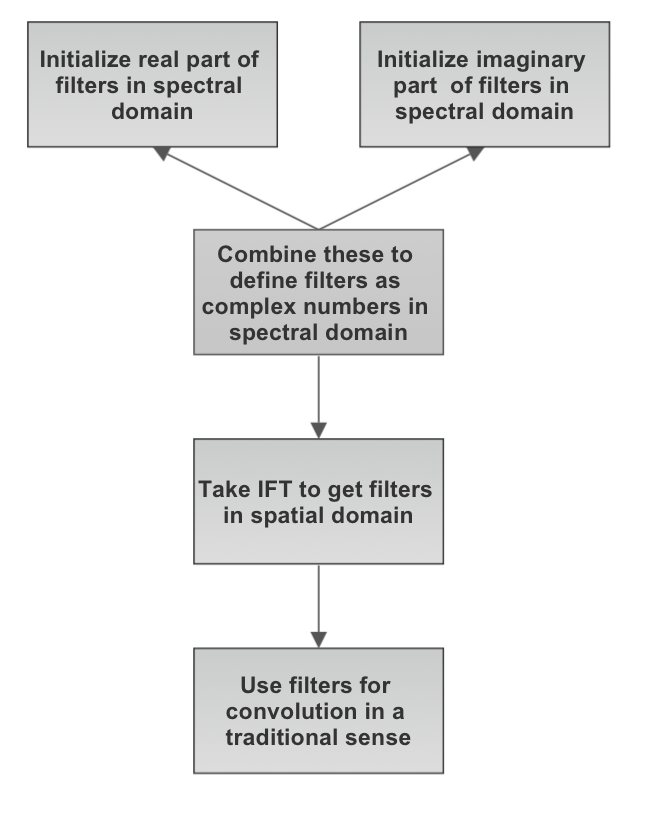
\includegraphics[width=250pt]{images/fc_spectral_param.png}
  \caption{Process for implementing spectral parameterization of CNN filters}
  \label{fig:spec_param}
\end{figure}

We implemented this proposal in TensorFlow by writing a custom convolutional layer class where the Variables (TensorFlow's learned parameters) correspond to the complex DFT coefficients instead of the filter weights.

\subsubsection{Spectral Pooling}

In most CNN architectures, the operation of the network gradually transforms an input image with 3 channels (R, G, and B values) and a large height and weight dimension (e.g. 3 x 32 x 32 or 3 x 224 x 224) to an output "image" consisting of a large (e.g., 512) number of channels and a small (e.g. 5x5, 3x3, or even 1x1) number of height and weight "pixels". Different CNN architectures achieve this in different ways, but one common approach is to use max-pooling to downsample the image periodically; for example, after every convolutional layer, or after every other convolutional layer, max-pooling may be used to cut the height and weight of the image roughly in half. With spectral pooling, the dimensionality reduction is instead performed by:
\begin{itemize}
\item Computing the two-dimensional DFT of the input tensor for each input channel
\item Truncating the resulting frequency matrix to the desired output dimensionality
\item Computing the inverse DFT of the truncated frequency matrix to obtain the output tensor for the given channel
\end{itemize}

\begin{figure}[ht]
\centering
  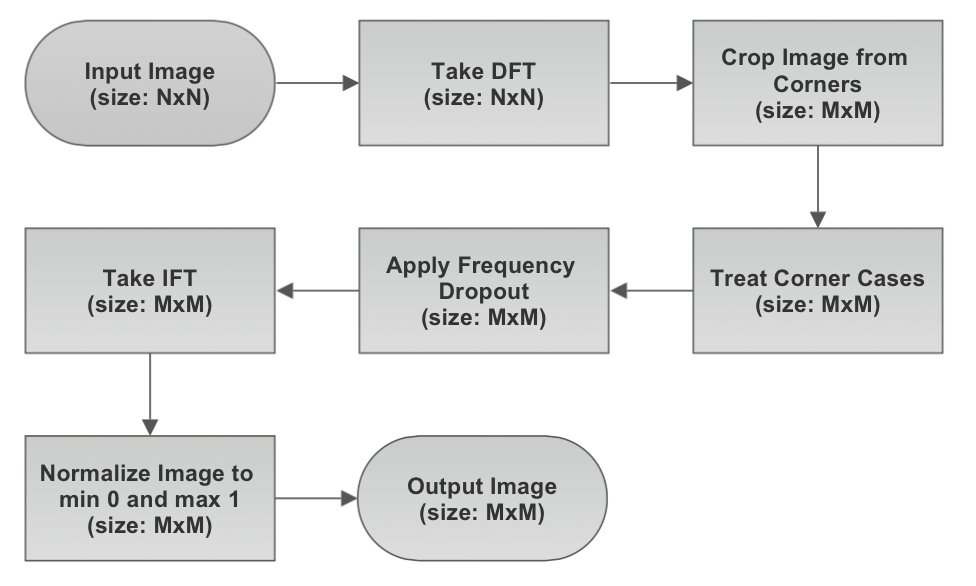
\includegraphics[width=250pt]{images/fc_spectral_pool.png}
  \caption{Process for implementing spectral pooling}
  \label{fig:spec_pool}
\end{figure}

A detailed description of the process can be found in the flowchart shown in Figure \ref{fig:spec_pool}. The truncation operation requires careful attention to detail in order to produce a real-valued output tensor. The DFT of a real-valued signal in the spatial domain obeys certain complex symmetries in the frequency domain; specifically, F[s, t] is the complex conjugate of F[-s, -t]; and, for a finite frequency matrix, if (s,t) and (-s,t) coincide modulo the dimension of the matrix, then F[s,t] must be real-valued; for example, the DC component, F[0,0] must be real valued, and for a 16 x 16 frequency matrix, F[8,8], F[0,8] and F[8,0] must also be real-valued. As a result, when an even-numbered output dimension is desired, the input frequency matrix cannot simply be truncated; the complex symmetries governing the original frequency matrix are not the same as the ones governing the truncated matrix. The paper refers to the need to handle these corner cases carefully but does not include the algorithm itself.

We implemented this proposal in TensorFlow by writing a custom spectral pooling function and layer class that always produces a truncated frequency matrix obeying the required complex symmetries. As with max-pooling, this layer has no learned parameters.

The pseudocode for spectral pooling as as follows. The index slices are using Python conventions.

\begin{itemize}
    \item Input: A 2-D, NxN Fourier transform matrix of complex coefficients where the DC component is located in the [0,0] top-left corner of the matrix
    \item Output: A 2-D, MxM (M $<$ N) Fourier transform matrix of complex coefficients where the DC component is located in the [0,0] top-left corner of the matrix
    \item If M is odd:
    \begin{itemize}
        \item KeepDim = (M-1) // 2
        \item TopLeft = Input[:KeepDim+1, :KeepDim+1]
        \item TopRight = Input[:KeepDim+1, -KeepDim:]
        \item BottomLeft = Input[-KeepDim:, :KeepDim+1]
        \item BottomRight = Input[-KeepDim:, -KeepDim:]
        \item Output $\leftarrow$ Combine TopLeft, TopRight, BottomLeft, BottomRight
    \end{itemize}
    \item Otherwise:
    \begin{itemize}
        \item KeepDim = M // 2
        \item TopLeft = Input[:KeepDim, :KeepDim]
        \item TopRight = Input[:KeepDim, -(KeepDim-1):]
        \item BottomLeft = Input[-(KeepDim-1):, :KeepDim]
        \item BottomRight = Input[-(KeepDim-1):, -(KeepDim-1):]
        \item MiddleColumn = Average of Input[:,KeepDim] and Input[:,-KeepDim]
        \item MiddleRow = Average of Input[KeepDim, :] and Input[-KeepDim, :]
        \item MiddlePoint = Average of Input[+/-KeepDim, +/-KeepDim]
        \item Output $\leftarrow$ Combine TopLeft, TopRight, BottomLeft, BottomRight, MiddleColumn, MiddleRow, and MiddlePoint
    \end{itemize}
\end{itemize}

The resulting truncated frequency matrix will always have the correct complex symmetries required such that its inverse Fourier transform will be real-valued.

The architecture of our spectrally-pooled CNN is described in Figure \ref{fig:cnn_arch}. The TensorFlow network diagram is shown in Figure \ref{fig:tb_graph}.

\begin{figure}[ht]
\centering
  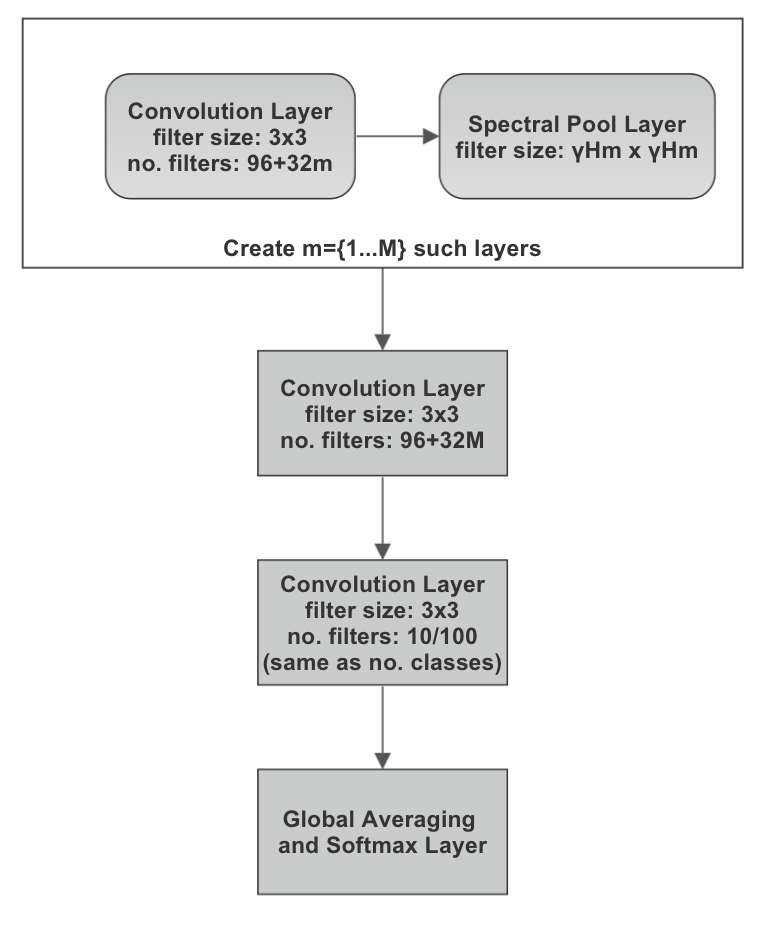
\includegraphics[width=200pt]{images/fc_cnn_arch.png}
  \caption{CNN with Spectral Pooling Architecture}
  \label{fig:cnn_arch}
\end{figure}

\begin{figure}[h]
\centering
  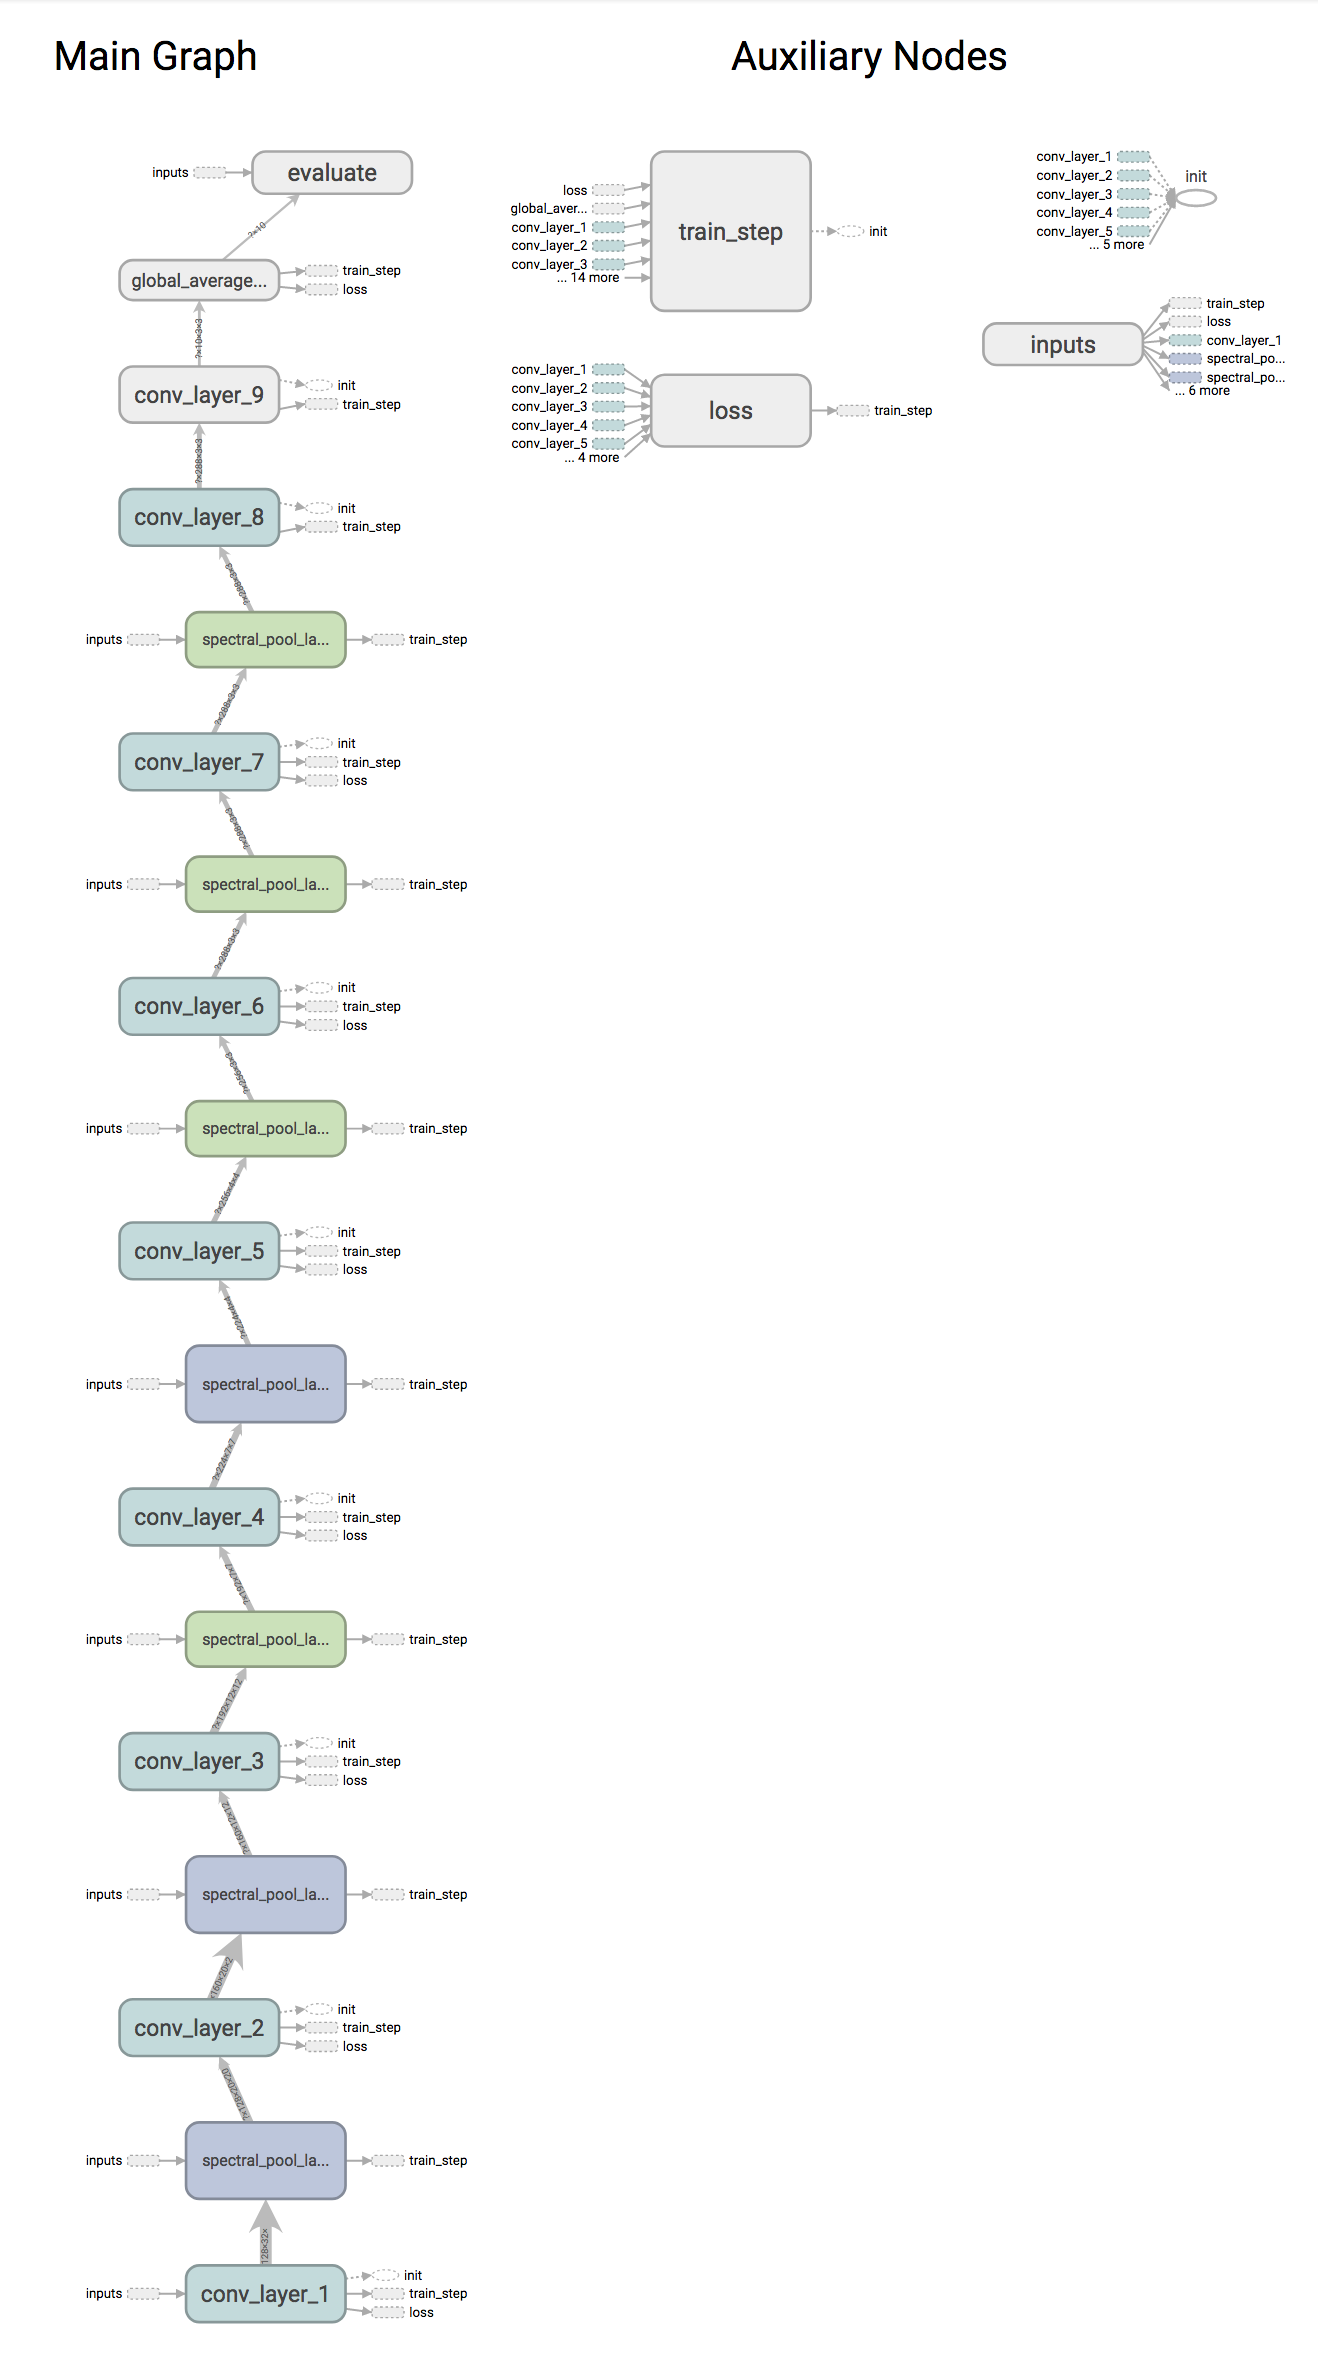
\includegraphics[width=200pt]{images/Architecture_10.png}
  \caption{TensorFlow Computational Graph}
  \label{fig:tb_graph}
\end{figure}

\subsubsection{Frequency Dropout}

This proposal is related to spectral pooling and is implemented in the same class, but serves a different purpose. The frequency matrix is computed for each input channel as before, but instead of being truncated to a smaller dimensionality, a brick-wall low-pass filter is instead applied: the higher frequencies are simply set to zero. The cutoff frequency for the filter is chosen randomly for each minibatch as a method of regularization. In the paper, this regularization is applied as part of the spectral pooling operation.

We implemented this proposal in TensorFlow by writing a function to perform the required filtering and incorporating the function into the spectral pooling layer. The pseudo-code for implementing frequency dropout is as below:
\begin{itemize}
    \item Input: Fourier transform matrix of complex coefficients of size MxM, with the DC component located in the top-left corner [0,0] of the matrix
    \item Output: Fourier transform matrix of complex coefficients of size MxM, with the DC component located in the top left corner [0,0] of the matrix, where all frequencies above a cutoff threshold T are set to zero
    \item Create a dropout mask matrix which is equal to zero if either the row or the column is greater than T and less than (M-T)
    \item Output $\leftarrow$ Input * DropoutMask
\end{itemize}

\subsection{Result Replication}

We attempted to reproduce the three key results of the original paper. The impressive classification rates in the original paper required an intense hyperparameter optimization over six separate hyperparameter dimensions that would have required more computational resources than we had available for this project, but the authors report most of the results of their optimization. For the parameters where they reported optimal results, we used those and attempted to search over the others. For the other two key results, we followed their methodology as closely as possible.

\subsubsection{Information Preservation}
We attempt to justify the key claim of using spectral pooling, i.e. higher information retrieval in the same number of dimensions. For this purpose, we first replicate Figure 2 of the original paper in Figure \ref{fig:fig2_gray}. Here, a 256x256 image is taken as input and max pooled images are compared with spectrally pooled images for increasing order of reduction from right to left. We can clearly see that spectral pooling retains more information. For instance, for the image on the extreme, a 64x64 max-pool looks nowhere close to a face but keeping just 8 frequencies still maintains the structure of a face.

\begin{figure}[ht]
\centering
  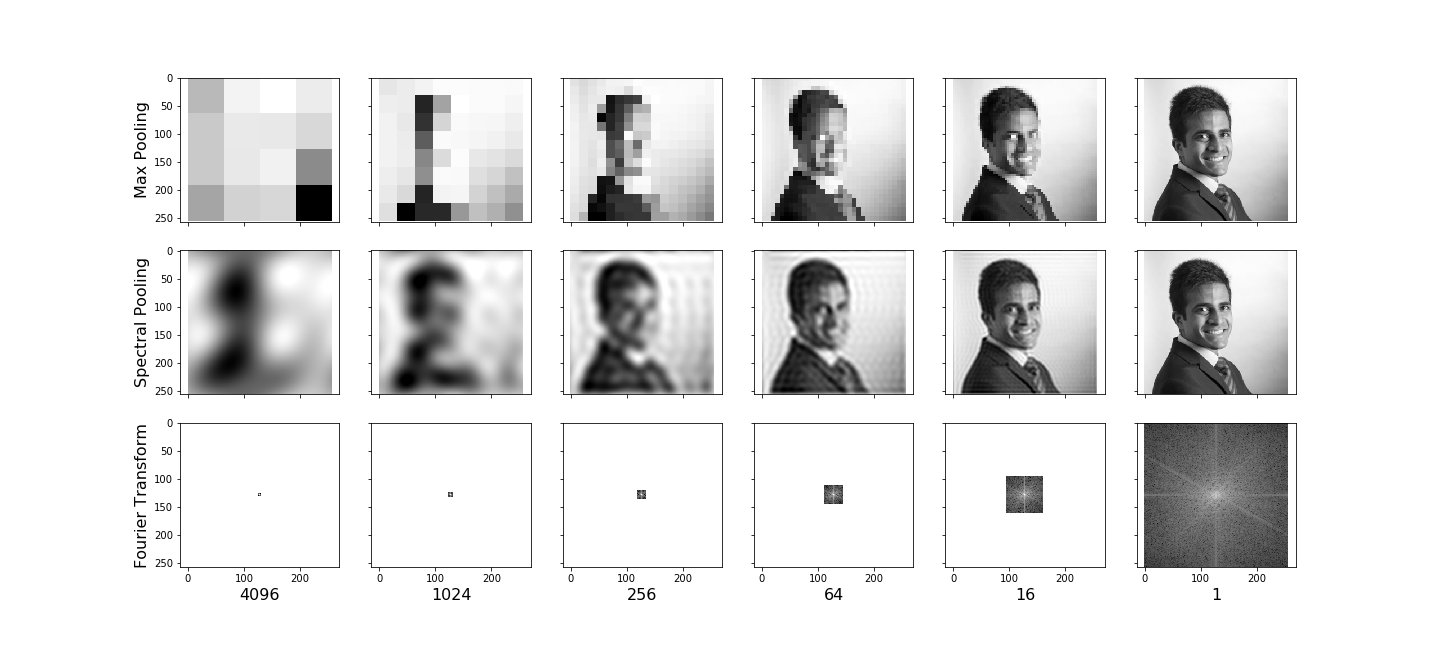
\includegraphics[width=250pt]{images/Figure2_Grayscale_Grid_Pooling.png}
  \caption{Higher information retrieval in spectral pooling as compared to max pooling (grayscale image)}
  \label{fig:fig2_gray}
\end{figure}

We did a similar analysis using the RGB version of the image and found similar results as shown in figure \ref{fig:fig2_color}.

\begin{figure}[ht]
\centering
  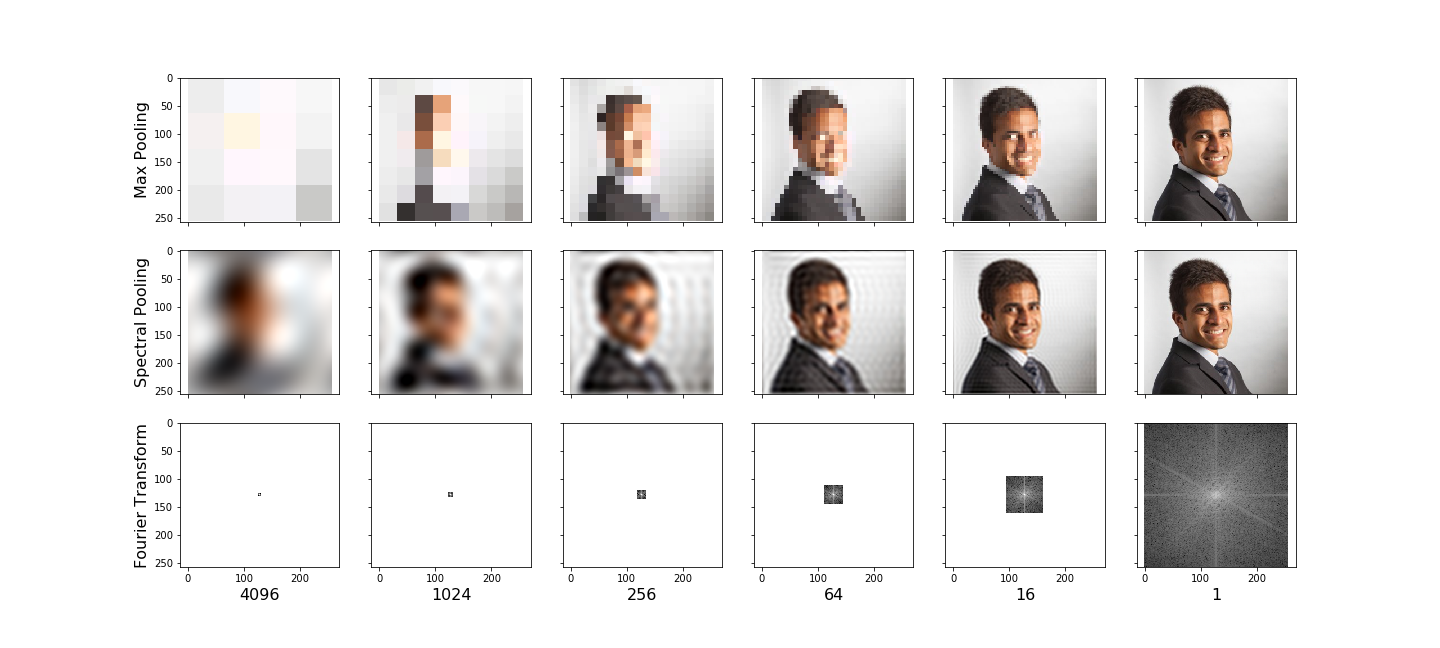
\includegraphics[width=250pt]{images/Figure2_RGB_Grid_Pooling.png}
  \caption{Higher information retrieval in spectral pooling as compared to max pooling (RGB image)}
  \label{fig:fig2_color}
\end{figure}

We also validated spectral pooling's higher information preservation by comparing the original image with the pooled image using max-pooling vs. spectral pooling. The results are shown in Figure \ref{fig:preserve}, where the x-axis shows the percentage of parameters kept and the y-axis shows the mean squared loss of the difference of original image vs modified image, normalized by the loss of the original image. This analysis has been run on the CIFAR-10 dataset. Please note that in the original paper, the validation set of Imagenet data was used, but the results are expected to be consistent irrespective of the dataset used.

\begin{figure}[ht]
\centering
  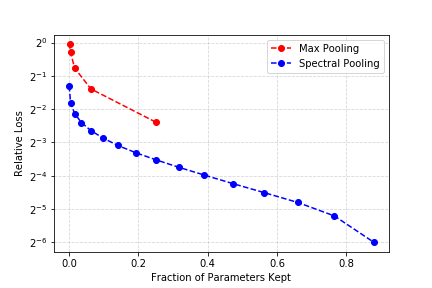
\includegraphics[width=250pt]{images/Figure4_Approximation_Loss.png}
  \caption{Comparison of the norm of the difference in original vs pooled images, showing higher information preservation in spectral pooling}
  \label{fig:preserve}
\end{figure}

\subsubsection{Spectral Pooling and Frequency Dropout for Traditionally Parameterized CNNs} \label{ssec:spec_pool_architecture}

We implemented a CNN class implementing the architecture specified in section 5.1 of the original paper. This architecture begins with M pairs of alternating layers of convolutional and spectral-pooling/frequency dropout layers, followed by a 1x1 convolutional layer with multiple filters, a 1x1 convolutional layer outputting the number of target classes, finally followed by a global averaging layer \cite{global_average} over which the softmax was computed for classification. The optimal hyperparameters which were not specified in the original paper were the number of layers and the weight decay rate. We performed hyperparameter search over a subsample of CIFAR-10 dataset \cite{cifar10} to identify the optimal parameters. As we used the Adam optimizer \cite{adam} instead of SGD with momentum, we added the initial learning rate and the dimensionality decay rate gamma to the set of hyperparameters over which we searched. We anneal the learning rate by 50\% after every 10 epochs. We randomly chose parameters on a log scale for the L2 norm and the learning rate and on a uniform scale for gamma and the number of layers M. We ran this search in parallel across multiple GPU instances and trained the network on the full datasets once the optimal hyperparameters had been identified. In addition to the random hyperparameter search, we also attempted to identify good hyperparameters by manually tuning.

\subsubsection{Optimization Convergence Speed}

To test the convergence speed of spectral parameterization, we created two new CNN architectures - deep and generic. The deep architecture is defined in the paper as two 96-filter convolutional layers, a 3x3 stride-2 max pool, three 192-filter convolutional layers, a 3x3 stride-2 max pool, a 192-filter 1x1 convolutional layer, a 10-filter 1x1 convolutional layer, and a global averaging layer. The generic architecture is a more standard CNN, with a 96-filter convolutional layer, 3x3 stride-2 max pool, 192-filter convolutional layer, 3x3 stride-2 max pool, then fully connected layers with sizes of 1024 and 512. Both architectures end with a softmax to compute the probabilities of each sample belonging to each of the 10 classes. We also tested with the spectral pooling architecture described in section \ref{ssec:spec_pool_architecture}, using M=3 layers and the optimal parameters presented in the original paper. For each of these three architectures, we trained 4 different configurations - 3x3 filters with spectrally parameterized conv weights, 3x3 filters with standard conv weights, and the same thing with 5x5 filters.

With all of our architectures defined, we used a standard training procedure, feeding mini-batches of 128 images through the network before computing and applying the gradient updates in an effort to minimize the loss (which was the sum of the cross entropy and l2 losses). We added vertical translations and horizontal flips after each epoch to increase the difficulty of training, as the paper indicates. For the models with spectral parameterization, we used the spectral convolution layer that was described in section \ref{ssec:spec_conv_layer}. The paper mentioned that they used a Bayesian optimizer to find the best hyperparameter values, but they did not actually state what those values were for the generic and deep architectures, so we hand-tuned the networks on small samples of the training data before training on the larger dataset. Due to the number of models involved with this test and the computational intensity that spectral pooling and spectral parameterization add, we opted to train them on just one of the five batches of CIFAR10 data (i.e. 10,000 of the 50,000 samples in the training set), and even that took 12 hours on a Google Cloud GPU. The results of this test are discussed in section 5.1.3.



\section{Results}

\subsection{Project Results and Comparison}

\subsubsection{Information Preservation}

Figure \ref{fig:preserve} shows a plot of the average information dissipation for the CIFAR-10 dataset. The y-axis displays the L2 error normalized by the norm of the input images.

The figure from the original paper is similar. Our plot was produced using the CIFAR-10 dataset instead of the ImageNet validation set, which is most likely responsible for any differences seen here. The ImageNet images are much larger, with an average resolution of approximately 475x400 pixels (depending on the year of the dataset in question) whereas the CIFAR images are only 32x32. We believe that our results substantially validate the claim of the original paper that spectral pooling preserves information in the original image files well.

\subsubsection{Spectral Pooling and Frequency Dropout for Traditionally Parameterized CNNs}

The best classification error rates we obtained for the CIFAR-10 and CIFAR-100 datasets were 18.76\% and 51.83\%, respectively. These were obtained with the following hyperparameters:

\begin{itemize}
\item M (number of spectral pooling layers): 6 for CIFAR 10, 4 for CIFAR 100
\item L2 Norm: 3e-4 for CIFAR 10, 1e-4 for CIFAR 100
\item $\gamma$ (dimensionality reduction at each spectral pooling layer: 0.79
\item Initial learning rate: 1e-3
\end{itemize}

Both of these results were improvements on the results of our hyperparameter search; the best results obtained by random search were 27.63\% for CIFAR-10 and 66.68\% for CIFAR-100, respectively. The random search parameters appeared to start overfitting the data quite early; their training curve is shown in Figure \ref{fig:train_curve}.

\begin{figure}
\centering
  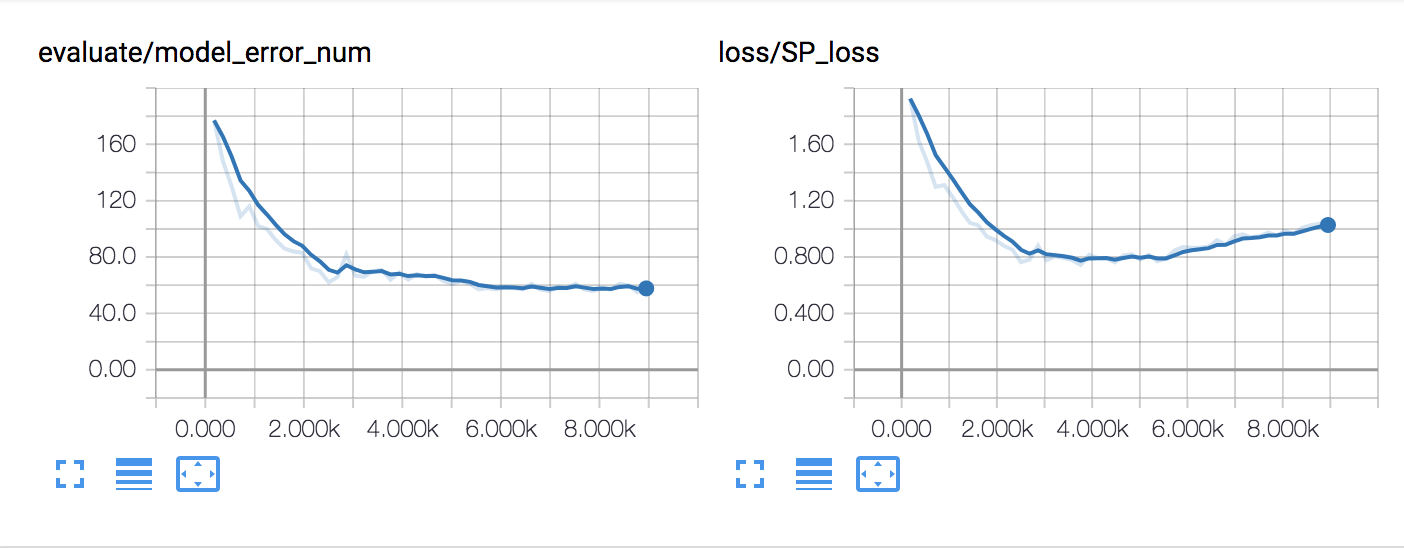
\includegraphics[width=200pt]{images/Training_Curve_10.png}
  \caption{Training Curve from Optimal Random-Search Hyperparameters}
  \label{fig:train_curve}
\end{figure}

The original paper reports results of 8.6\% for CIFAR 10 and 31.6\% for CIFAR 100, respectively; therefore, our results were significantly worse than the results reported by the paper's authors.

\subsubsection{Optimization Convergence Speed}

In the original paper, the authors claimed that spectral parameterization consistently improved the number of epochs it took to reach convergence by a factor of 2.2 to 5.1, depending on the architecture. While our speed-up factors do not exactly match those of the original paper, our tests did reveal the benefits of using spectral parameterization. In figure 9, we have plotted the training accuracies across epochs for each of our models. The exact values of the error rates are less important than the relative shapes of the two curves in any one plot. The generic architecture converged to minimal training error in an almost identical fashion both with and without spectral parameterization, but the other two architectures showed significant improvements through the use of spectral parameterization.

The deep model shows an improvement in convergence for both the 3x3 and 5x5 filter sizes. The deep-5 experiences a 1.3x speed-up (not quite as large as the 4.8x speed-up reported in the original) while the deep-3 model shows a drastic improvement through the use of spectral parameterization — it achieves a 5.4x speed-up, while the original paper reports a 2.2x speed-up. The deep-3 network with spectral parameterization not only greatly sped up convergence, it also unlocked a minimal error rate that was nearly 20 percentage points better than the deep-3 without spectral parameterization.

The results for the spectral pooling architecture are even more drastic. Due to time constraints, we had to reduce the size of the spectral pooling architecture and only use 3 convolutional+spectral pooling layer pairs. This led to our non-spectrally parameterized models struggling to learn the training set well, with each struggling to get below 50 percent error rate, while the models with spectral parameterization blow past 50 percent in fewer than 10 epochs and proceed to hit 0 percent by the end of the training. This leads to speed-up factors of 18.8 and 16.7 -- much higher than the values reported in the original paper.

\begin{figure}
\centering
  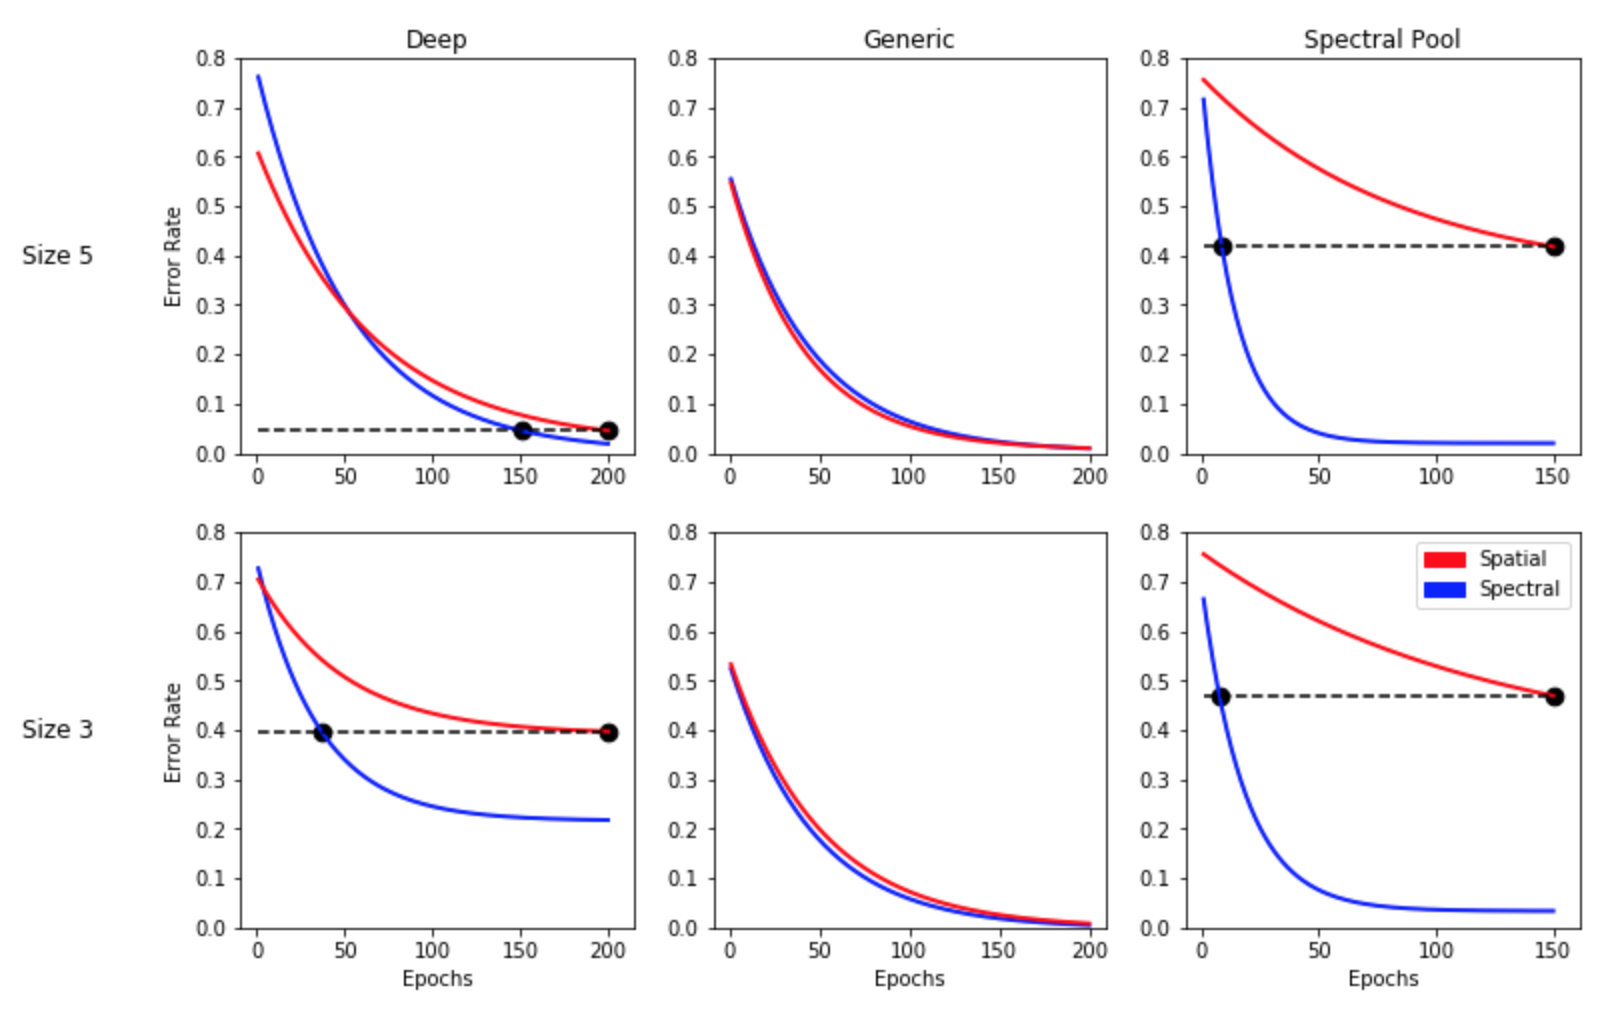
\includegraphics[width=250pt]{images/Spectral_Param_Training_Curves.png}
  \caption{Error rates for various architectures in optimization convergence speed test.}
  \label{fig:spectral_param_training_curves}
\end{figure}

\begin{table}[h!]
  \begin{center}
    \caption{Comparison of original paper's speed-up factors vs. ours.}
    \label{tab:Optimization Convergence}
    \begin{tabular}{c|c|c|c}
      \textbf{Architecture} & \textbf{Filter Size} & \textbf{Original Speed-up} & \textbf{Our Speed-up}\\
      \hline
      Deep & 3x3 & 2.2 & 5.4\\
      Deep & 5x5 & 4.8 & 1.3\\
      Generic & 3x3 & 2.2 & 0\\
      Generic & 5x5 & 5.1 & 0\\
      Spectral Pool & 3x3 & 2.4 & 18.8\\
      Spectral Pool & 5x5 & 4.8 & 16.7\\
    \end{tabular}
  \end{center}
\end{table}

\subsection{Insights Gained}

Implementing the proposals of this paper and attempting to replicate their results was an extremely enjoyable and educational project. None of us had a background in signal processing before attempting this project and we are grateful to have had the opportunity to learn about the Fourier transform and its applications in image processing. It was disappointing that we were not able to replicate the impressive results obtained by the authors. However, after thinking about the proposals and their implications, we have certain theories for why our results with these techniques were essentially equivalent to the results obtained with standard CNNs.

When we were first discussing the paper before we began to implement the proposals, our theory for why the spectrally parameterized filters would be easier to optimize than the traditionally parameters filters was the DFT was a mysterious nonlinear operation and that the resulting parameters had "nicer" derivatives than the standard parameters. As an analogy, even though the tanh function and the logistic sigmoid are nearly identical, the difference in the range of the two functions makes it much easier for stochastic gradient descent to optimize networks using tanh for the nonlinearity than those with employing the sigmoid function. It is now obvious to us that the Fourier transform is a linear transform and the DFT coefficients are linear combinations of the filter weights, so this theory about the derivatives does not seem plausible.

Despite this, we did indeed find that the spectrally parameterized networks often converge faster in practice. Although we don't have a particularly satisfying explanation for this, we assume, as do the original authors, that this is a result of the of the form of the parameter updates used by the Adam optimizer. As the original authors write, "[T]his parametrization corresponds to a rotation to a more meaningful axis alignment, where the number of relevant elements has been significantly reduced. Since modern optimizers implement update rules that consist of adaptive element-wise rescaling, they are able to leverage this axis alignment by making large updates to a small number of elements." We can see in the deep architecture with 3x3 filters and both spectral pooling architectures, the spectrally parameterized model not only converges to the non-spectral minimum error rate much more quickly, it also achieves a distinctly lower error rate, conceivably because the optimizer was able to explore a different space with the axis alignment provided by the spectral parameterization.

Another insight, related to the spectral pooling operation, involves this choice of downsampling operation and its effects on the image content. As the images in both the original paper and ours demonstrate, it is clearly true that we can still easily understand an image after a fairly drastic dimensionality reduction through spectral pooling. However, there is certain important information that is lost by discarding the high-frequency content of an image. For example, edge detection, which is typically one of the first filters learned by a CNN, is essentially equivalent to discarding all of the low-frequency content of an image! As a result, it is not so clear why the spectral pooling operation would be the best way of downsampling the image, particularly as it is transformed through the network. In fact, it is somewhat akin to average-pooling, which has empirically not proved as successful in most CNN architectures as max-pooling.

Finally, it is not clear to us why the frequency dropout technique should have been as successful as a regularization technique as the authors found. The traditional dropout operation has a clear interpretation as a way of forcing the network to act as an ensemble with shared weights and the statistical properties of ensembles are well known to produce superior results. Although there may be a sound theoretical explanation for why frequency dropout is successful at regularizing a CNN, we were not able to come up with one.

\section{Conclusion}

Spectral pooling is a downsampling technique that can gradually reduce the dimensionality of an image while maintaining a close approximation to the original image. However, we were not able to replicate the authors' finding that spectral pooling and the related technique of frequency dropout were able to sufficiently regularize the network on their own in order to achieve classification rates on the CIFAR-10 and CIFAR-100 that were substantially superior to previously reported techniques. Finally, despite not matching the authors' error rates exactly, we did show that in some cases, the Adam optimizer did converge in substantially fewer epochs when optimizing a network parameterized by the spectral coefficients of the convolutional filters as opposed to the filter weights themselves.

\section{Acknowledgements}

We are grateful to Stanford Professor Brad Osgood and to Stanford University for the outstanding series of lecture videos, The Fourier Transform and its Applications, which are available on YouTube. We are also grateful to Google and the TensorFlow authors and contributors, who have developed and open-sourced a library that makes it possible to implement these complex proposals in an extraordinarily efficient way that correctly and automatically implements differentiation and backpropagation for us while allowing us to take advantage of GPUs. We would like to thank Michael Shell, who created the LaTeX template that we used to produce this report. Finally, we would like to thank Professor Kostic for making this fascinating paper available as one of the options for our final project!


% add bib
\bibliographystyle{IEEEtranS}
\bibliography{bibfile}

\section{Appendix}

\subsection{Individual Student Contributions}

\end{document}
